\subsection{Universidad de Sydney - Australia}
Presentamos en la siguiente tabla los resultados obtenidos del último monitoreo.

\bigskip
\begin{tabular}{ | l | c | c | c | c |}
 
  \hline                 
  Hop & IP &  RTT promedio (s)  & deltaRTT promedio & Ubicación\\
  \hline
  1  &  192.168.0.1  &  0.00317819338096  &  0.00317819338096 & Argentina - Buenos Aires\\
  \hline
  2  &  200.89.165.169  &  0.0273115007501  &  0.0241333073691 & Argentina - Buenos Aires\\
  \hline
  3  &  200.89.165.5  &  0.0295196944161  &  0.00220819366606 & Argentina - Buenos Aires\\
  \hline
  4  &  200.89.165.250  &  0.0303499635897  &  0.000830269173572 & Argentina - Buenos Aires\\
  \hline
  5  &  207.136.166.241  &  0.0279953793476  &  0 & Estados Unidos\\
  \hline
  6  &  67.16.139.18  &  0.15700549953  &  0.129010120183 & Estados Unidos - Illinois\\
  \hline
  7  &  64.208.27.102  &  0.151270602879  &  0 & Estados Unidos\\
  \hline
  8  &  129.250.3.172  &  0.15870277662  &  0.00743217374149 & Estados Unidos - Colorado\\
  \hline
  9  &  129.250.2.219  &  0.176934030495  &  0.0182312538749 & Estados Unidos - Colorado\\
  \hline
  10  &  129.250.7.69  &  0.185023287409  &  0.00808925691404 & Estados Unidos - Colorado\\
  \hline
  11  &  129.250.3.123  &  0.185811053765  &  0.000787766356217 & Estados Unidos - Colorado\\
  \hline
  12  &  204.1.253.166  &  0.185876883959  &  0.0000658301930679 & Estados Unidos - California\\
  \hline
  13  &  202.158.194.172  &  0.3106533885  &  0.124776504542 & Australia - New South Wales\\
  \hline
  14  &  113.197.15.68  &  0.305794251593  &  0 & Australia - New South Wales\\
  \hline
  15  &  113.197.15.66  &  0.331599779819  &  0.0258055282267 & Australia - New South Wales\\
  \hline
  16  &  113.197.15.62  &  0.330528166733  &  0 & Australia - New South Wales\\
  \hline
  17  &  113.197.15.13  &  0.330654288593  &  0.000126121859801 & Australia - New South Wales\\
  \hline
  18  &  138.44.5.47  &  0.337141043261  &  0.00648675466839 & Australia\\
  \hline
  19  &  129.78.5.11  &  0.337009869124  &  0 & Australia - Sydney\\
  \hline
  20  &  129.78.5.11  &  0.337688013127  &  0.000678144003216 & Australia - Sydney\\
  \hline
  21  &  129.78.5.11  &  0.336762147514  &  0 & Australia - Sydney\\
  \hline
  22  &  129.78.5.11  &  0.338513030818  &  0.00175088330319 & Australia - Sydney\\
  \hline
  23  &  129.78.5.11  &  0.336039300028  &  0 & Australia - Sydney\\
  \hline
  24  &  129.78.5.11  &  0.339367595158  &  0.00332829513048 & Australia - Sydney\\
  \hline
\end{tabular}
\bigskip

Con estos datos hemos obtenido que los $\Delta$ $RTT$ siguen una distribución normal con una probabilidad del 99,5$\%$ ($\alpha$ $=$ 0,005).
Se ha realizado el test de $Grubbs$ y nos ha devuelto que los $outliers$ se encuentran en los saltos 6 y 13.\\

A continuación mostramos que ocurre con los $RTT$ promedio de cada salto y con los $zScore$ promedio de cada salto:

\begin{figure}[H]
\centering
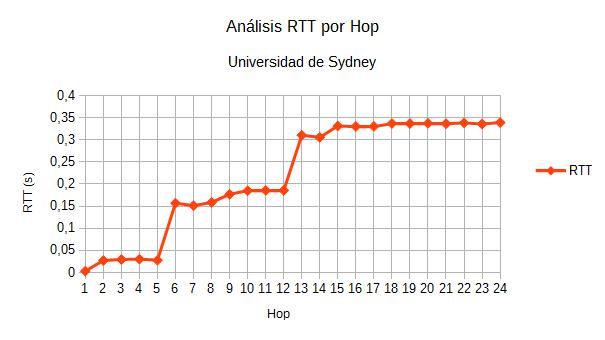
\includegraphics[width=1\textwidth]{graficos/rTT_Australia.jpg}
\caption{RTT promedio por hop - Universidad de Sydney}
\label{Australia_rtt}
\end{figure}

\begin{figure}[H]
\centering
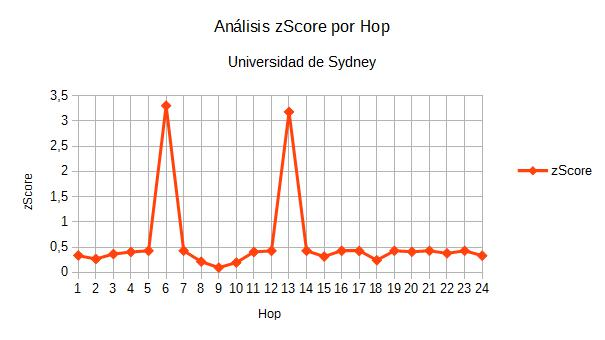
\includegraphics[width=1\textwidth]{graficos/zScore_Australia.jpg}
\caption{zScore promedio por hop - Universidad de Sydney}
\label{Australia_zs}
\end{figure}

Tanto en la tabla como en los gráficos se puede observar claramente que hubo dos $outliers$, uno de los cuales fue el esperado salto transatlántico: 
desde Estados Unidos hacia Australia (salto 13). Dicho enlace submarino (con un $RTT$ promedio que supera los 300 ms), contrasta con los $RTT$ de los hops anteriores 
que se encontraban por debajo de los 200 ms. En este caso la ubicación obtenida de la herramienta ha acompañado los datos.\\

El otro $outlier$ detectado (salto 6) se produce cuando se viaja desde Argentina hacia Estados Unidos, nuevamente nos es extraño que no se detecta en el primer 
hop hasta dicho país, sino en el segundo. Seguimos bajo la suposición que la primera $IP$ que se geolocaliza en Estados Unidos, la 207.136.166.241, 
tiene un servidor alojado en Argentina o en algún país limítrofe, ya que el $RTT$ promedio hasta allí es muy bajo (similiar a host situados en Argentina).\\ 

A continuación hemos trazado en un mapa la ruta de nuestro host hasta el host destino ubicado en Australia:
\begin{figure}[H]
\centering
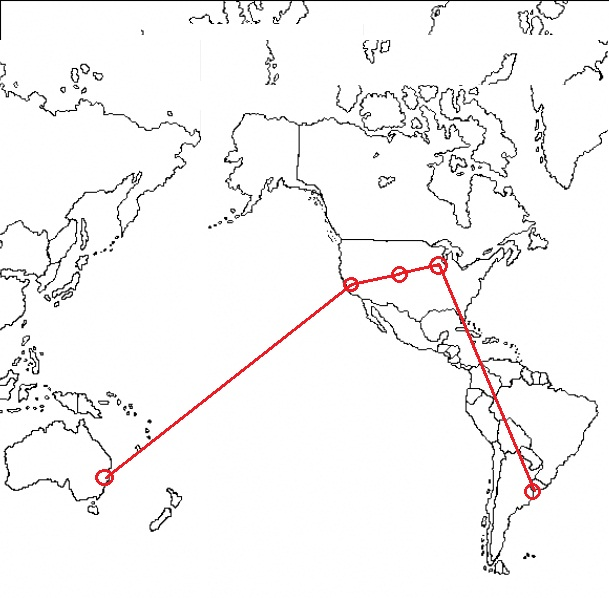
\includegraphics[width=0.8\textwidth]{graficos/mapa_australia.jpg}
\caption{Ruta en Internet - Universidad de Sydney}
\label{australia_zs}
\end{figure}

Éste es un claro ejemplo de lo ineficente que pueden llegar a ser las rutas en internet. 
Tal vez se deba a la falta de enlaces entre América Latina y Australia, ya que un recorrido recto podría haber llegado a ahorrar casi la mitad del tiempo.